\documentclass[17pt,compress]{beamer}
\usepackage{beamerthemesplit}
\mode<presentation>
{
  \usetheme{Warsaw}
  \setbeamercovered{transparent}
  \setbeamertemplate{navigation symbols}{}
}
% Taken from Fernando's slides.
\usepackage{ae,aecompl}
\usepackage[scaled=.95]{helvet}

\usepackage[english]{babel}
\usepackage[latin1]{inputenc}
\usepackage[T1]{fontenc}

\newcounter{saveenumi}
\newcommand{\seti}{\setcounter{saveenumi}{\value{enumi}}}
\newcommand{\conti}{\setcounter{enumi}{\value{saveenumi}}}

\definecolor{blue}{rgb}{0.16,0.32,0.75}
\setbeamercolor{structure}{fg=blue}
\author[FOSSEE]{}
\institute[IIT Bombay]{}
\date[]{}
% \setbeamercovered{transparent}

% theme split
\usepackage{verbatim}
\newenvironment{colorverbatim}[1][]%
{%
\color{blue}
\verbatim
}%
{%
\endverbatim
}%

\usepackage{mathpazo,courier,euler}
\usepackage{listings}
\lstset{language=sh,
    basicstyle=\ttfamily\bfseries,
  showstringspaces=false,
  keywordstyle=\color{black}\bfseries}

% logo
\logo{
\includegraphics[height=1.30 cm]{3t-logo.pdf}}
\logo{
\includegraphics[height=1.30 cm]{fossee-logo.png}

\hspace{7.5cm}

\includegraphics[scale=0.3]{fossee-logo.png}\\
\hspace{281pt}

\includegraphics[scale=0.80]{3t-logo.pdf}}

\begin{document}

\sffamily \bfseries
\title
[Using Plot Interactively]
{Python - Using Plot Interactively}
\author
[FOSSEE, IIT - Bombay]
{\small Talk to a Teacher\\{\color{blue}\url{http://spoken-tutorial.org}}\\National Mission on Education
 through ICT\\{\color{blue}\url{http://sakshat.ac.in}} \\[0.5cm]{\tiny Script by: Hardik ghaghada \\ Naration by: Hardik Ghaghada \\ 13 August 2015}}

% slide 1
\begin{frame}
   \titlepage
\end{frame}
%%%%%%%%%%%%%%%%%%%%%%%%%%%%%%%%%%%%%%%%%%%%%%%%%%%%%%%%%%%%%%%%%%%%%%%%%%%%%%%%
\begin{frame}
\frametitle{Objectives}
\label{sec-2}
In this tutorial, we will learn -\pause
\begin{itemize}
\item Create simple plots of mathematical functions. \pause
\item Use the Figure window to study plots better.
\end{itemize}
\end{frame}
%%%%%%%%%%%%%%%%%%%%%%%%%%%%%%%%%%%%%%%%%%%%%%%%%%%%%%%%%%%%%%%%%%%%%%%%%%%%%%%%
\begin{frame}
\frametitle{System Specifications}\pause
\begin{itemize}
\item Slackware Linux 14.1\pause
\item \texttt{Python 2.7.5} \pause
\item \texttt{IPython 2.3.0}
\end{itemize}
\end{frame}
%%%%%%%%%%%%%%%%%%%%%%%%%%%%%%%%%%%%%%%%%%%%%%%%%%%%%%%%%%%%%%%%%%%%%%%%%%%%%%%%
\begin{frame}
\frametitle{Pre-requisites}
Spoken tutorial on -
\begin{itemize}
\item  getting started with \texttt{ipython~}
\end{itemize}
\end{frame}
%%%%%%%%%%%%%%%%%%%%%%%%%%%%%%%%%%%%%%%%%%%%%%%%%%%%%%%%%%%%%%%%%%%%%%%%%%%%%%%%

\begin{frame}
\frametitle{Error if matplotlib is not installed}
\label{sec-3}
\begin{itemize}
\item `ERROR: matplotlib could NOT be imported! Starting normal IPython.'\\
\label{sec-3_1}%
\end{itemize} % ends low level
\end{frame}
%%%%%%%%%%%%%%%%%%%%%%%%%%%%%%%%%%%%%%%%%%%%%%%%%%%%%%%%%%%%%%%%%%%%%%%%%%%%%%%%
\begin{frame}
\frametitle{Plot UI}
\label{sec-4}
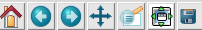
\includegraphics[height=0.12in, interpolate=true]{buttons.png}
\begin{itemize}
\item Save
\item Zoom
\item Move axis
\item Back and Forward Button
\item Home
\end{itemize}
\end{frame}
%%%%%%%%%%%%%%%%%%%%%%%%%%%%%%%%%%%%%%%%%%%%%%%%%%%%%%%%%%%%%%%%%%%%%%%%%%%%%%%%
\begin{frame}
\frametitle{Exercise 1}
\label{sec-5}
Plot \texttt{(sin(x)*sin(x))/x}.\pause
\begin{enumerate}
\item Save the plot as sinsquarebyx.pdf in pdf format.\pause
\item Zoom and find the maxima.\pause
\item Bring it back to initial position.
\end{enumerate}
\end{frame}
%%%%%%%%%%%%%%%%%%%%%%%%%%%%%%%%%%%%%%%%%%%%%%%%%%%%%%%%%%%%%%%%%%%%%%%%%%%%%%%%
\begin{frame}
\frametitle{Summary}
\label{sec-6.1}
In this tutorial, we have learnt to -\pause
\begin{itemize}
\item Start \texttt{ipython} with \texttt{pylab}.
\item Use the \texttt{linspace} function to create equally spaced points in a region.
\item Find the length of sequences using \texttt{len} function.
\end{itemize}
\end{frame}
%%%%%%%%%%%%%%%%%%%%%%%%%%%%%%%%%%%%%%%%%%%%%%%%%%%%%%%%%%%%%%%%%%%%%%%%%%%%%%%%
\begin{frame}
\frametitle{Summary contd..}
\label{sec-6.2}
\begin{itemize}
\item Plot mathematical functions using \texttt{plot}.
\item Clear drawing area using \texttt{clf}.
\item Use the UI of plot
\begin{itemize}
\item Save
\item Zoom
\item Move axis
\item Back and Forward Button
\item Home
\end{itemize}
\end{itemize}
\end{frame}
%%%%%%%%%%%%%%%%%%%%%%%%%%%%%%%%%%%%%%%%%%%%%%%%%%%%%%%%%%%%%%%%%%%%%%%%%%%%%%%%
\begin{frame}
\frametitle{Evaluation}
\label{sec-7.1}
\begin{enumerate}
\item Create 100 equally spaced points between -pi/2 and pi/2\pause
\item How to find the length of a sequence.
	\seti
\end{enumerate}
\end{frame}
%%%%%%%%%%%%%%%%%%%%%%%%%%%%%%%%%%%%%%%%%%%%%%%%%%%%%%%%%%%%%%%%%%%%%%%%%%%%%%%%
\begin{frame}
\frametitle{Evaluation contd..}
\label{sec-7.2}
\begin{enumerate}
	\conti
\item What will the command \texttt{linspace(-pi,pi,100)} do?\pause
\begin{itemize}
\begin{footnotesize}
\item returns 100 evenly spaced samples from -pi to pi\pause
\item returns 100 evenly spaced samples from -pi to pi excluding pi but including -pi\pause
\item returns 100 evenly spaced samples from -pi to pi excluding -pi but including pi\pause
\item returns 100 evenly spaced samples from -pi to pi including both -pi \& pi
\end{footnotesize}
\end{itemize}
\end{enumerate}
\end{frame}
%%%%%%%%%%%%%%%%%%%%%%%%%%%%%%%%%%%%%%%%%%%%%%%%%%%%%%%%%%%%%%%%%%%%%%%%%%%%%%%%
\begin{frame}
\frametitle{Solutions\ldots{}}
\label{sec-8}
\begin{enumerate}
\item \texttt{linspace(-pi/2,pi/2,100)}\pause
\item \texttt{len(sequence\_name)}\pause
\item returns 100 evenly spaced samples from -pi to pi including both -pi and pi
\end{enumerate}
\end{frame}
%%%%%%%%%%%%%%%%%%%%%%%%%%%%%%%%%%%%%%%%%%%%%%%%%%%%%%%%%%%%%%%%%%%%%%%%%%%%%%%%
\begin{frame}
\frametitle{FOSSEE}
{\color{blue}Free and Open-source Software for \\Science and Engineering Education} \\
\begin{itemize}
\item Goal - enabling all to use open source software tools
\item For more details, please visit {\color{blue}\url{http://fossee.in/}}
\end{itemize}
\end{frame}
%%%%%%%%%%%%%%%%%%%%%%%%%%%%%%%%%%%%%%%%%%%%%%%%%%%%%%%%%%%%%%%%%%%%%%%%%%%%%%%%
\begin{frame}
\frametitle{About the Spoken Tutorial Project}
\begin{itemize}
\item Watch the video available at {\color{blue}http://spoken-tutorial.org /What\_is\_a\_Spoken\_Tutorial}
\item It summarises the Spoken Tutorial project \pause
\item If you do not have good bandwidth, you can download and watch it
\end{itemize}
\end{frame}
%%%%%%%%%%%%%%%%%%%%%%%%%%%%%%%%%%%%%%%%%%%%%%%%%%%%%%%%%%%%%%%%%%%%%%%%%%%%%%%%
\begin{frame}
\frametitle{Spoken Tutorial Workshops}The Spoken Tutorial Project Team 
\begin{itemize}
\item Conducts workshops using spoken tutorials 
\item Gives certificates to those who pass an online test 
\item For more details, please write to \\ \hspace {0.5cm}{\color{blue}contact@spoken-tutorial.org}
\end{itemize}
\end{frame}
%%%%%%%%%%%%%%%%%%%%%%%%%%%%%%%%%%%%%%%%%%%%%%%%%%%%%%%%%%%%%%%%%%%%%%%%%%%%%%%%
\begin{frame}
\frametitle{Acknowledgements}
\begin{itemize}
\item Spoken Tutorial Project is a part of the Talk to a Teacher  project 
\item It is supported by the National Mission on Education through  ICT, MHRD, Government of India 
\item More information on this Mission is available at: \\{\color{blue}http://spoken-tutorial.org /NMEICT-Intro}
\end{itemize}
\end{frame}
%%%%%%%%%%%%%%%%%%%%%%%%%%%%%%%%%%%%%%%%%%%%%%%%%%%%%%%%%%%%%%%%%%%%%%%%%%%%%%%%
\begin{frame}

  \begin{block}{}
  \begin{center}
  \textcolor{blue}{\Large THANK YOU!} 
  \end{center}
  \end{block}
\begin{block}{}
  \begin{center}
    For more Information, visit our website\\
    \url{http://fossee.in/}
  \end{center}  
  \end{block}
\end{frame}
%%%%%%%%%%%%%%%%%%%%%%%%%%%%%%%%%%%%%%%%%%%%%%%%%%%%%%%%%%%%%%%%%%%%%%%%%%%%%%%%
\end{document}
